The concept of crypto-currency has overcame many problems in fiat currency. On the other hand, there are some economical applications which are well-shaped and implemented in traditional fiat markets; among them: Option trading, Arbitrage, Loan, Bond, Auction, etc. But in crypto-currency, the field is open into the new ideas and contains lots of implementation challenges. 

By the invention of Ethereum smart contracts, so many decentralized financial (DeFi) applications were made which results in a rapidly growth of the crypto-currency market capital and decentralized backed tokens. In order to show the economical willingness towards the subject, some financial application implementation are mentioned below:

% Some developed solutions for applying these traditional economical applications to the world of crypto-currencies are:

% Some of the reputed DeFi applications are Compound, Maker DAO

% There are some developed solutions for applying these traditional economical applications to the world of crypto-currency.Here are some examples from


\begin{itemize}
    \item \textbf{ACO}: A protocol for decentralized and non-custodial trading of options \cite{aco}.
    \item \textbf{Jelly Swap}: A peer to peer trading tool across different blockchains using atomic swaps \cite{jelly}.
    \item \textbf{Uniswap}: A fully decentralized on-chain protocol for token exchanges on Ethereum that uses liquidity pools instead of order books \cite{uniswap}.
    \item \textbf{Aave}: An open source and non-custodial protocol to earn interest on depositing and borrowing assets \cite{aave}.
    \item \textbf{MakerDAO}: A decentralized credit platform on Ethereum that supports Dai, a stablecoin whose value is pegged to USD and backed in ETH or BAT \cite{maker}. 
    \item \textbf{Compound}: An open-source money market protocol on Ethereum that lets users lend or borrow assets against collateral \cite{compound}. 
    \item \textbf{Atomic Loan}: A lending platform that accepts trustless BTC collateral via custom Bitcoin scripts \cite{atomicLoan}. 
    \item \textbf{DAI}: A decentralized stablecoin soft-pegged to the US Dollar \cite{maker}. 
    \item \textbf{WBTC}: An ERC20 token that is backed 1:1 by bitcoin and opened the gate of trading bitcoin under ethereum blockchain \cite{wbtc}.
    \item \textbf{dYdX}: An non-custodial trading platform on Ethereum geared toward experienced traders \cite{dydx}. 
    
\end{itemize}

For showing the growing investment interest in financial derivatives of crypto currencies, we can consider Fig.~\ref{fig:TVL-ACO} and \ref{fig:TVL-Uniswap} which are the overview of the money (in USD) locked in Uniswap and ACO and their fluctuations during the recent three months:
\begin{figure}
    \centering
    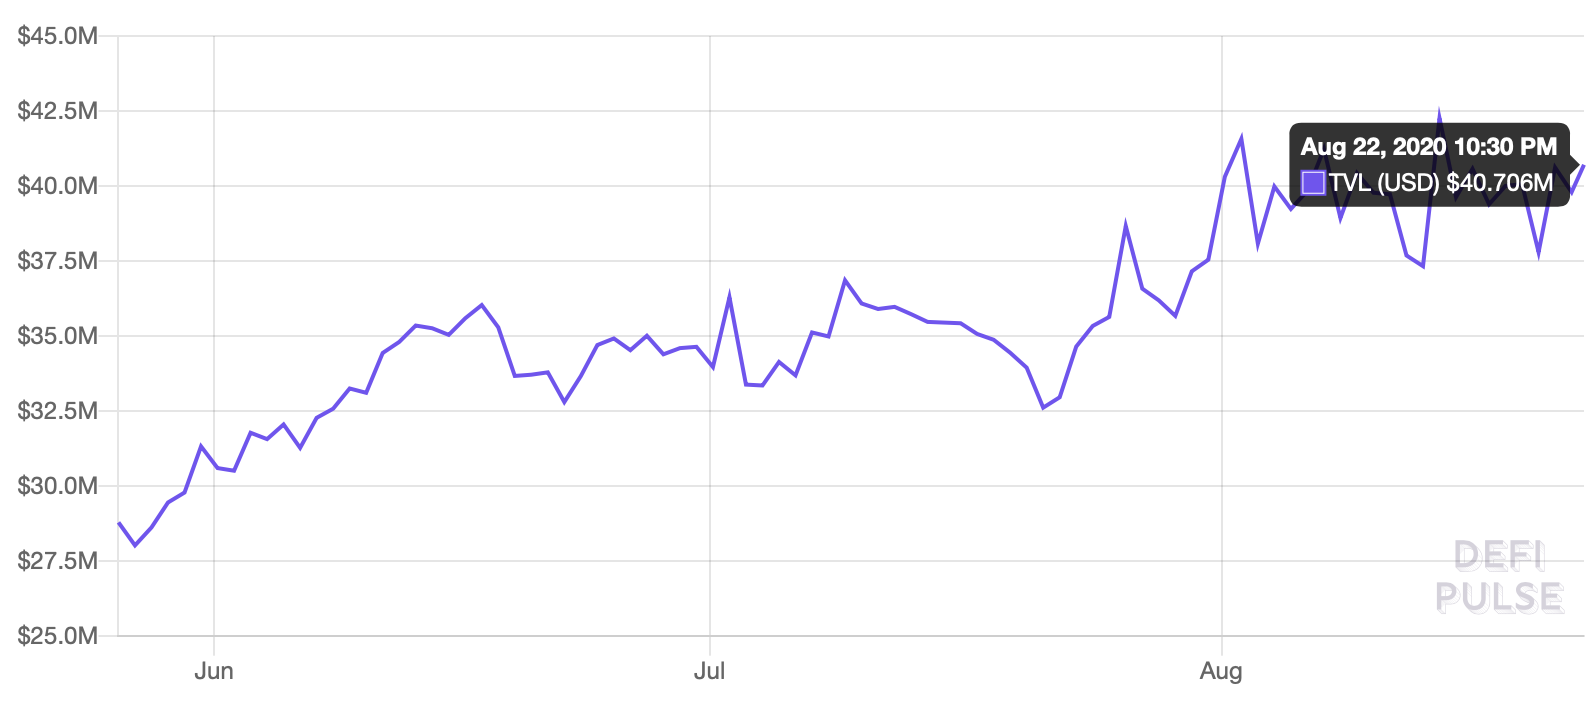
\includegraphics[width=\textwidth]{figures/dydx.png}
    \caption{Total value locked (USD) in dydx \cite{dydx-cap}. Currently more than 40 M\$}
    \label{fig:TVL-ACO}
\end{figure}
\begin{figure}
    \centering
    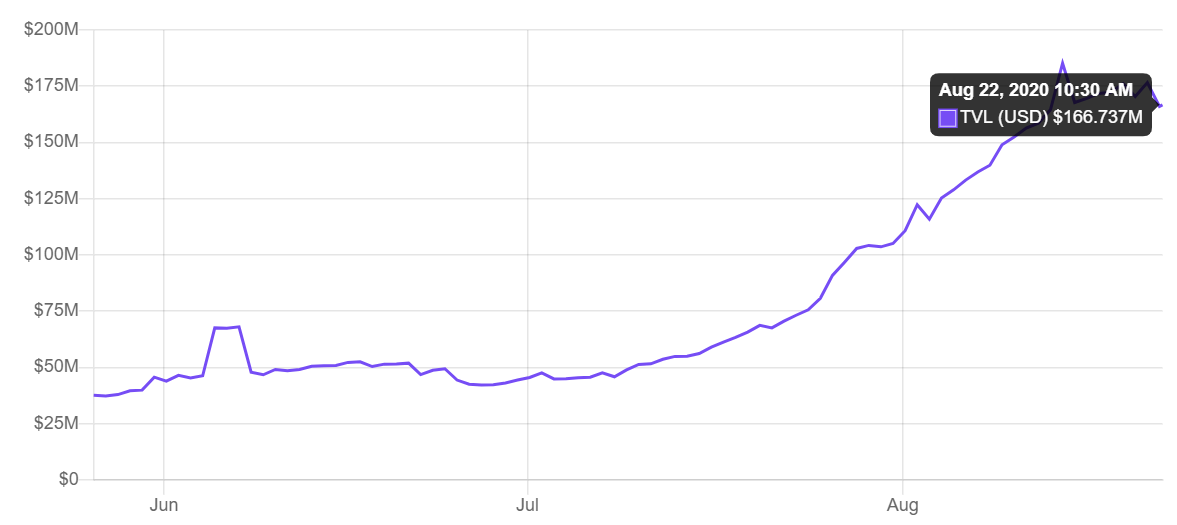
\includegraphics[width=\textwidth]{figures/TVL(USD)-uniswap-90.png}
    \caption{total value locked (USD) in Uniswap \cite{uniswap-cap}. Currently more than 166 M\$}
    \label{fig:TVL-Uniswap}
\end{figure}


By the given information we can conclude that the market of crypto currencies and specially loan, option and inter-blockchain swaps are being demanded these days more than before. 

In this work, we target this opportunity and designed fully decentralized future market applications which in addition to ethereum blockchain, work on first generation blockchains like bitcoin which does not support high level scripting languages. Our protocols and procedures only need Hash Time Lock Contracts as their building block and they do not rely on any oracle or third party interference. Moreover, for the first time in cryptocurrency market, we offer an atomic unsecured crosschain bond service. 
The rest of this paper is organized as follows. In Section~\ref{sec:swaption}, we review concepts about atomic swaption and design a general model of atomic swaption for furthur usage. In Section~\ref{sec:abcd}, we extend our model to make the ABCD. Finally, in Section~\ref{sec:arbitrage}, we adopt our model to build arbitrage opportunity in the swaption market.



% Most of mentioned systems have one thing in common: they are implemented for a turing complete bock chain and with the aid of smart contracts.


% \begin{tabular}{||c c c c c c||} 
%  \hline
%  BTC & ETH & DAI & AE & WBTC & USDC \\ [0.5ex] 
%  \hline\hline
%  20709.97 & 19216.02 & 9598.86 & 10226.57 & 209.33 & 3756.75 \\ [1ex] 
%  \hline
% \end{tabular}


 
